% Please use the skeleton file you have received in the 
% invitation-to-submit email, where your data are already
% filled in. Otherwise please make sure you insert your 
% data according to the instructions in PoSauthmanual.pdf
\documentclass{PoS}

\usepackage{multirow} 

\newcommand{\CLs}{\ensuremath{CL_\mathrm{s}}}
\newcommand{\CLb}{\ensuremath{CL_\mathrm{b}}}
\newcommand{\CLsb}{\ensuremath{CL_\mathrm{s+b}}}

%\newcommand{\GeV}{\ensuremath{\mathrm{Ge\kern -0.1em V}}}
%\newcommand{\TeV}{\ensuremath{\mathrm{Te\kern -0.1em V}}}
%\newcommand{\TeVcc}{\ensuremath{\,\mathrm{Te\kern -0.1em V\!/c}^2}}
%\newcommand{\GeVcc}{\ensuremath{\,\mathrm{Ge\kern -0.1em V\!/c}^2}}
%\newcommand{\MeVcc}{\ensuremath{\,\mathrm{Me\kern -0.1em V\!/c}^2}}
%\newcommand{\GeVc}{\ensuremath{\mathrm{Ge\kern -0.1em V}\!/c}}
\newcommand{\nanob}{\mbox{{\rm ~nb}~}}
\newcommand{\fb}{\ensuremath{\mathrm{fb}}}
\newcommand{\pb}{\ensuremath{\mathrm{pb}}}
\newcommand{\ifb}{\ensuremath{\mathrm{fb^{-1}}}}
\newcommand{\ipb}{\ensuremath{\mathrm{pb^{-1}}}}
\newcommand{\grad}{\ensuremath{^{\circ}}}
%
% Special user made math symbols
%
\newcommand{\lsim}{\raisebox{-1.5mm}{$\:\stackrel{\textstyle{<}}{\textstyle{\sim}}\:$}}
\newcommand{\gsim}{\raisebox{-1.5mm}{$\:\stackrel{\textstyle{>}}{\textstyle{\sim}}\:$}}

% particles

\newcommand{\pipm}{\ensuremath{\pi^{\pm}}}
\newcommand{\pizero}{\ensuremath{\pi^{0}}}
\newcommand{\Hi}{\ensuremath{\mathrm{H}}}
\newcommand{\W}{\ensuremath{\mathrm{W}}}
\newcommand{\Wjets}{\ensuremath{\mathrm{W+jets}}}
\newcommand{\Zjets}{\ensuremath{\mathrm{Z+jets}}}
\newcommand{\Wt}{\ensuremath{\mathrm{Wt}}}
\newcommand{\Wstar}{\ensuremath{\mathrm{W}^{*}}}
\newcommand{\Wparenthesisstar}{\ensuremath{\mathrm{W}^{(*)}}}
\newcommand{\WW}{\ensuremath{\W^+\W^-}}
\newcommand{\Z}{\ensuremath{\mathrm{Z}}}
\newcommand{\Zstar}{\ensuremath{\mathrm{Z}^{*}}}
\newcommand{\ZZ}{\ensuremath{\Z\Z}}
\newcommand{\WZ}{\ensuremath{\W\Z}}
\newcommand{\El}{\ensuremath{\mathrm{\mathrm{e}}}}
\newcommand{\Elp}{\ensuremath{\mathrm{\mathrm{e}}^{+}}}
\newcommand{\Elm}{\ensuremath{\mathrm{\mathrm{e}}^{-}}}
\newcommand{\Elpm}{\ensuremath{\mathrm{\mathrm{e}}^{\pm}}}
\newcommand{\Elmp}{\ensuremath{\mathrm{\mathrm{e}}^{\mp}}}
\newcommand{\M}{\ensuremath{\mu}}
\newcommand{\Mp}{\ensuremath{\mu^{+}}}
\newcommand{\Mm}{\ensuremath{\mu^{-}}}
\newcommand{\Mpm}{\ensuremath{\mu^{\pm}}}
\newcommand{\Mmp}{\ensuremath{\mu^{\mp}}}
\newcommand{\Tau}{\ensuremath{\tau}}
\newcommand{\Pgt}{\ensuremath{\tau}}
\newcommand{\Nu}{\ensuremath{\nu}}
\newcommand{\Nubar}{\ensuremath{\bar{\nu}}}
\newcommand{\Lep}{\ensuremath{\mathrm{\ell}}}
\newcommand{\Lepp}{\ensuremath{\mathrm{\ell}^{+}}}
\newcommand{\Lepm}{\ensuremath{\mathrm{\ell}^{-}}}
\newcommand{\Lprime}{\ensuremath{\Lep^{\prime}}}
\newcommand{\Prot}{\ensuremath{\mathrm{p}}}
\newcommand{\Pbar}{\ensuremath{\bar{\mathrm{p}}}}
\newcommand{\PP}{\Prot\Prot}
\newcommand{\PPbar}{\Prot\Pbar}
\newcommand{\ttbar}{\ensuremath{\mathrm{t}\bar{\mathrm{t}}}}
\newcommand{\qq}{\ensuremath{\mathrm{q}\mathrm{q}}}
\newcommand{\bbbar}{\ensuremath{\mathrm{b}\bar{\mathrm{b}}}}
\newcommand{\Wtb}{\ensuremath{\W\mathrm{t}\mathrm{b}}}
\newcommand{\Top}{\ensuremath{\mathrm{t}}}
\newcommand{\Bot}{\ensuremath{\mathrm{b}}}
\newcommand{\Atop}{\ensuremath{\bar{\mathrm{t}}}}
\newcommand{\Abot}{\ensuremath{\bar{\mathrm{b}}}}
% arrow
\newcommand{\To}{\ensuremath{\rightarrow}}

% masses
\newcommand{\mHi}{\ensuremath{m_{\mathrm{H}}}}
\newcommand{\mW}{\ensuremath{m_{\mathrm{W}}}}
\newcommand{\mZ}{\ensuremath{m_{\mathrm{Z}}}}
\newcommand{\mll}{\ensuremath{m_{\Lep\Lep}}}

% kinematics
\newcommand{\pt}{\ensuremath{p_\mathrm{T}}}
\newcommand{\ptveto}{\ensuremath{\pt^\mathrm{veto}}}
\newcommand{\ptl}{\ensuremath{p_\perp^{\Lep}}}
\newcommand{\ptlmax}{\ensuremath{p_{\mathrm{T}}^{\Lep,\mathrm{max}}}}
\newcommand{\ptlmin}{\ensuremath{p_{\mathrm{T}}^{\Lep,\mathrm{min}}}}
\newcommand{\ETm}{\ensuremath{E_{\mathrm{T}}^{\mathrm{miss}}}}
\newcommand{\met}{\ETm}
\newcommand{\MET}{\ETm}
\newcommand{\MT}{\ensuremath{M_\mathrm{T}}}
\newcommand{\delphill}{\ensuremath{\Delta\phi_{\Lep\Lep}}}
\newcommand{\deletall}{\ensuremath{\Delta\eta_{\Lep\Lep}}}
\newcommand{\delphimetl}{\ensuremath{\Delta\phi_{\met\Lep}}}
\newcommand{\delphimetll}{\ensuremath{\Delta\phi_{\met\Lep\Lep}}}
\newcommand{\Et}{\ensuremath{E_\mathrm{T}}}
\newcommand{\delR}{\ensuremath{\Delta R}}
\newcommand{\Eta}{\ensuremath{\eta}}
\newcommand{\GAMMA}{\ensuremath{\gamma}}

%efficiencies
\newcommand{\effsig}{\ensuremath{\varepsilon_{\mathrm{bkg}}^{\mathrm{S}}}}
\newcommand{\effnorm}{\ensuremath{\varepsilon_{\mathrm{bkg}}^{\mathrm{N}}}}
\newcommand{\Nsig}{\ensuremath{N_{\mathrm{bkg}}^{\mathrm{S}}}}
\newcommand{\Nnorm}{\ensuremath{N_{\mathrm{bkg}}^{\mathrm{N}}}}

% processes
\newcommand{\dyee}{\ensuremath{\mathrm{\Z}/\GAMMA^*\mathrm{\to e^+e^-}}}
\newcommand{\dymm}{\ensuremath{\mathrm{\Z/}\GAMMA^*\to\mu^+\mu^-}}
\newcommand{\dytt}{\ensuremath{\mathrm{\Z}/\GAMMA^* \to\tau^+\tau^-}}
\newcommand{\dyll}{\ensuremath{\mathrm{\Z}/\GAMMA^*\mathrm{\to \ell^+\ell^-}}}
\newcommand{\zee}{\ensuremath{\mathrm{\Z\to e^+e^-}}}
\newcommand{\zmm}{\ensuremath{\mathrm{\Z}\to\mu^+\mu^-}}
\newcommand{\ztt}{\ensuremath{\mathrm{\Z}\to\tau^+\tau^-}}
\newcommand{\zll}{\ensuremath{\mathrm{\Z\to \ell^+\ell^-}}}
%\newcommand{\ttbar}{\ensuremath{t\bar{t}}}
\newcommand{\ppww}{\ensuremath{pp \to W^+W^-}}
\newcommand{\wwlnln}{\ensuremath{W^+W^-\to \ell^+\nu \ell^-\bar{\nu}}}
\newcommand{\ww}{\ensuremath{WW}}
\newcommand{\wwpm}{\ensuremath{W^+W^-}}
\newcommand{\hww}{\Hi\to\WW}
\newcommand{\wz}{\ensuremath{WZ}}
\newcommand{\zz}{\ensuremath{ZZ}}
\newcommand{\wgamma}{\ensuremath{\W\GAMMA}}
\newcommand{\wjets}{\ensuremath{W+}jets} 
\newcommand{\tw}{\ensuremath{\mathrm{t}\W}} 
\newcommand{\singletopt}{\ensuremath{t} ($t$-chan)} 
\newcommand{\singletops}{\ensuremath{t} ($s$-chan)} 

% units
\newcommand{\mus}{\ensuremath{\mu\mathrm{s}}}
\newcommand{\de}{\ensuremath{^\circ}}

%other 
\def\fixme{({\bf FixMe})}
\newcommand{\ee}{\ensuremath{ee}}
\newcommand{\emu}{\ensuremath{e\mu}}
\def\mm{\ensuremath{\mu\mu}}

% integrated luminosity
\newcommand{\usedLumi}{5.1 fb {\ensuremath{^{-1}}}}
\newcommand{\usedLumiWithSyst}{\ensuremath{5.1 \pm 0.2} fb {\ensuremath{^{-1}}}}


\title{Search for SM Higgs decaying to $WW\to \ell\nu\ell\nu$ and $\ell\nu~qq$ at CMS}

\ShortTitle{Search for SM Higgs decaying to WW to lvlv and lvqq at CMS}

\author{\speaker{Emanuele Di Marco}\\
       {\rm On behalf of the CMS Collaboration}\\
       California Institute of Technology\\
       E-mail: \email{emanuele.di.marco@cern.ch}}


\abstract{A search for the standard model Higgs boson decaying to
  W$^+$W$^-$.  The pp collisions data sample corresponds to an
  integrated luminosity of 5.1~fb$^{-1}$ at $\sqrt{s}$ = 7 TeV and
  5.1~fb$^{-1}$ at $\sqrt{s}$ = 8 TeV, collected by the CMS detector
  at the LHC.  The W$^+$W$^-$ candidates are selected in events in the
  fully leptonic or semi leptonic final state. Upper limits on the
  Higgs boson production relative to the standard model Higgs
  expectation are derived.  The standard model Higgs boson is excluded
  in the mass range 129--520~GeV at 95\% confidence level from the
  fully leptonic channel and in the mass ranges 260--460~GeV from the
  semi-leptonic channel.  A 1.6 $\sigma$ (2.4 $\sigma$) excess of events
  is observed (expected) for low Higgs boson masses which makes the
  observed limits weaker than the expected ones under the null
  hypothesis.}

\FullConference{36th International Conference on High Energy Physics,\\
		July 4-11, 2012\\
		Melbourne, Australia}


\begin{document}

\section{Introduction}
One of the open questions in the standard model (SM) of particle
physics is the origin of the masses of fundamental
particles. Within the SM, vector boson masses arise from the
spontaneous breaking of electroweak symmetry by the Higgs
field~\cite{Higgs1, Higgs2}.  The
existence of the associated field quantum, the Higgs boson, has yet to
be established experimentally. The discovery or the exclusion of the
SM Higgs boson is one of the central goals of the CERN Large Hadron
Collider (LHC) physics program.
%% Direct searches at the CERN $e^+e^-$ LEP collider set a limit on the
%% Higgs boson mass $m_{\Hi} > 114.4~GeV$ at 95\% confidence level
%% (CL)~\cite{LEPHIGGS}. Precision electroweak data constrain the mass of
%% the SM Higgs boson to be less than 158~GeV at 95\%
%% CL~\cite{EWK,2005ema}.  The SM Higgs boson is excluded at 95\% CL by
%% the Tevatron collider experiments in the mass range
%% 147--179~GeV~\cite{TEVHIGGS_2012} and by the ATLAS experiment in the
%% mass ranges 111.4--116.6, 119.4--122.1 and
%% 129.2--541~GeV~\cite{AtlasPaperCombination}.  Previous results from
%% the Compact Muon Solenoid (CMS) collaboration exclude the SM Higgs
%% boson in the mass ranges
%% 127.5--600~GeV~\cite{CmsMoriondCombination,CmsPaperCombination} at
%% 95\% CL.
In this conference I reported about the search for the Higgs boson in
the $\Hi \to \WW \to 2\ell 2\nu$ and $\Hi \to \WW \to \ell \nu 2q$
final states, where $\ell$ is a charged lepton, electron or muon,
$\nu$ a neutrino, and $q$ a quark.  The first analysis is performed in
the mass range 110--600~GeV, while the second, which needs a high
\pt\ lepton to trigger the \W\ decaying leptonically, is only
performed in the mass range 170--600~GeV.  The search discussed here
is performed using the data sample corresponding to
\usedLumiWithSyst\ of integrated luminosity collected in 2012 at a
center-of-mass energy of 8~TeV. Finally, the $\sqrt{s} = 7$ TeV data
sample is added to the analysis to obtain the combined 2011 and 2012
results.  The data collected by CMS detector, a multipurpose apparatus
designed to study high transverse momentum ($\pt$) physics processes
in proton-proton collisions (described in detail
in~\cite{CMSdetector}), are used.

%%%%%%%%%%%%%%%%%%%%%%%%%%%%%%%%%%%%%%%%%%%%%%%%%%%%%%%%%%%%%%%%%%%%%%%%%%%%%%%
\section{Physics objects for $\WW \to \ell\nu\ell\nu$ and $\WW \to \ell\nu qq$ event selection}
\label{sec:ww_evtsel}
%%%%%%%%%%%%%%%%%%%%%%%%%%%%%%%%%%%%%%%%%%%%%%%%%%%%%%%%%%%%%%%%%%%%%%%%%%%%%%%
The search strategy for $\hww\to\ell\nu\ell\nu$ is based on a
signature with two isolated, oppositely charged, high $\pt$ leptons
(electrons or muons) and large missing transverse momentum, $\MET$,
due to the undetected neutrinos. To improve the signal sensitivity,
the events are separated by jet multiplicity into three mutually
exclusive categories.  The search strategy for $\hww\to\ell\nu 2q$ is
based on the final state with one high $\pt$ lepton (electron or
muon), large \MET\ and two or three jets due to the hadronic decay of
the \W\ and one possible additional jet in the event. In the $\WW \to
\ell\nu\ell\nu$ analysis the events are selected by triggers which
require the presence of one or two high-$\pt$ electrons or muons.  For
the semi-leptonic channel, a suite of single lepton triggers mostly
using transverse momentum thresholds of 24 GeV for muons and 27 GeV
for electrons is used.

Muon candidates are identified using a selection similar to the one
described in~\cite{HWW2011}. Muons are required to be isolated to
distinguish between muon candidates from \W-boson decays and those
from QCD background processes, which are usually in or near jets. For
each muon candidate, the scalar sum of the transverse energy of all
particles compatible with originating from the primary vertex is
reconstructed in cones of several widths around the muon direction.
Electron candidates are identified using a multivariate approach based
on variables similar to those described in~\cite{egmpas} and
exploiting information from the tracker, the ECAL, and the combination
of these two detectors. Electrons are required to be isolated by
applying a threshold on the sum of the transverse energy of the
particles which are reconstructed in a cone around them.  For both
electrons and muons a correction is applied to account for the
contribution to the energy in the isolation cone from the pile-up
using the measured median energy density in the event. They are
required to originate from the primary vertex of the event.

Jets are reconstructed using the anti-$\mathrm{k_T}$ clustering
algorithm~\cite{antikt} with distance parameter $\Delta
\mathrm{R}=0.5$.  A similar
correction as for the lepton isolation is applied to account for the
contribution to the jet energy from the pile-up. Jet energy
corrections are applied as a function of the jet $\Et$ and
$\eta$.  A selection is applied to separate jets from
the primary interaction from those reconstructed due to energy
deposits associated with pile-up, based on the differences in the jet
shapes, in the relative multiplicity of charged and neutral components
and in the different fraction of transverse momentum which is carried
by the hardest components.  Within the tracker acceptance the jet
tracks are also required to be compatible with the primary
vertex. Events are classified according to the number of selected jets
with $\Et>30$ GeV and $|\eta|<$4.7.

In addition to high momentum isolated leptons and minimal jet activity
missing transverse momentum is present in signal events due to
$\W\to\ell\nu$ decays.  For the $\WW\to\ell\nu\ell\nu$ final state
with same-flavor leptons, a large background comes from Drell-Yan
process, where no real \MET\ is present. In this case a
\textit{projected}~$\MET$ variable is employed. It is equal to the
component of $\MET$ transverse to the nearest lepton if the difference
in azimuth between this lepton and the $\MET$ vector is less than
$\pi/2$. If there is no lepton within $\pi/2$ of the direction of
$\MET$ in azimuth, $\MET$ is used directly.  Since the
\textit{projected}~$\MET$ resolution is degraded by pile-up, the
minimum of two $\MET$ observables is used: the first includes all
reconstructed particles in the event, while the second uses only the
charged particles associated with the primary vertex.  In the
semi-leptonic final state, since the main background arises from
associated \W\ and jets production with real \MET, no projection is
needed.


%%%%%%%%%%%%%%%%%%%%%%%%%%%%%%%%%%%%%%%%%%%%%%%%%%%%%%%%%%%%%%%%%%%%%%%%%%%%%%%
\section{$\Hi \to \WW \to \ell\nu\ell\nu$ search strategy}
\label{sec:hww2l2nu}
%%%%%%%%%%%%%%%%%%%%%%%%%%%%%%%%%%%%%%%%%%%%%%%%%%%%%%%%%%%%%%%%%%%%%%%%%%%%%%%

Two oppositely charged lepton candidates are required, with $\pt >20$
GeV for the leading lepton ($\ptlmax$) and $\pt >10$ GeV for the
trailing lepton ($\ptlmin$).  Only electrons (muons) with $|\eta|
<$2.5 (2.4) are considered in the analysis.  Events with
\textit{projected}~$\MET$ above 20 GeV are selected for the analysis.
To suppress the top-quark background, a \textit{top tagging} technique
based on soft-muon and b-jet tagging~\cite{btag} is applied. The first
method is designed to veto events containing muons from b-quarks
coming from top-quark decays.  The second method uses b-jet tagging
algorithm which looks for tracks with large impact parameter within
jets.  A minimum dilepton transverse momentum ($\pt^{\ell\ell}$) of 45
GeV is required to reduce the $\Wjets$ background.  To reduce the
background from $\WZ$ production, any event that has a third lepton
passing the identification and isolation requirements is rejected. The
contribution from $\wgamma$ production, where the photon is
misidentified as an electron, is reduced by about 90\% in the
dielectron final state by $\GAMMA$ conversion rejection requirements.
The contribution from $\wgamma^{*}$ is reduced by the veto on the
presence of a third lepton and by isolation requirements.  The
background from low mass resonances is rejected by requiring a
dilepton mass ($\mll$) greater than 12 GeV.  The Drell-Yan process
produces same-flavor lepton pairs ($\Elp\Elm$ and $\Mp\Mm$). In order
to suppress this background, a few additional cuts are applied in the
same-flavor final states.  First, the resonant component of the
Drell-Yan production is rejected by requiring a dilepton mass outside
a 30 GeV window centered on the $\Z$ pole.  Then, the remaining
off-peak contribution is suppressed by exploiting different \MET-based
approaches depending on the number of jets and the Higgs mass
hypothesis.  At large Higgs masses ($\mHi > 140$ GeV), signal events
are associated with large \MET, thus it is sufficient to require the
minimum of the two \textit{projected}~$\MET$ variables to be greater
than 45 GeV. For $\mHi \leq 140$ GeV analysis, a dedicated
multivariate selection combining missing transverse momentum,
kinematic and topological variables, is used. In events with two jets
the dominant source of fake \MET\ is the mismeasurement of the
hadronic recoil, thus $\MET > 45$ GeV is sufficient.  Finally, the
momenta of the dilepton system and of the most energetic jet must not
be back-to-back in the transverse plane. These selections effectively
reduce the Drell-Yan background by three orders of magnitude, while
rejecting less than 50\% of the signal.

After applying the full set of selection criteria described in this
section, referred to as the $\WW$ selection, the observed yields in
data are 1594, 1186, and 1295 events in the 0-jet, 1-jet, and 2-jet
categories respectively. This sample is dominated by non-resonant
$\WW$ events.  To enhance the sensitivity to a Higgs boson signal, a
cut-based approach is chosen for the final Higgs selection. Because
the kinematics of signal events change as a function of the Higgs
mass, separate optimizations are performed for different $\mHi$
hypotheses. The extra requirements, designed to optimize the
sensitivity for a SM Higgs boson, are placed on $\ptlmax$, $\ptlmin$,
$\mll$, $\delphill$ and the transverse mass $m_\mathrm{T}$, defined as
$\sqrt{2 \pt^{\ell\ell} \MET (1-\cos\delphimetll)}$, where
$\delphimetll$ is the difference in azimuth between $\MET$ and the
transverse momentum of the dilepton system.  The $\delphill$ and
$\mll$ distributions in the 0-jet category, for a
$\mHi=125$ GeV SM Higgs boson and for the main backgrounds are shown
in Figure~\ref{fig:dphillHWW}.  The clear difference in the shape
between the $\Hi \to \WW$ and the non-resonant $\WW$ processes is due
to the spin-0 nature of the Higgs boson.

%----------------------------------------------------
\begin{figure}[htbp]
\begin{center}
   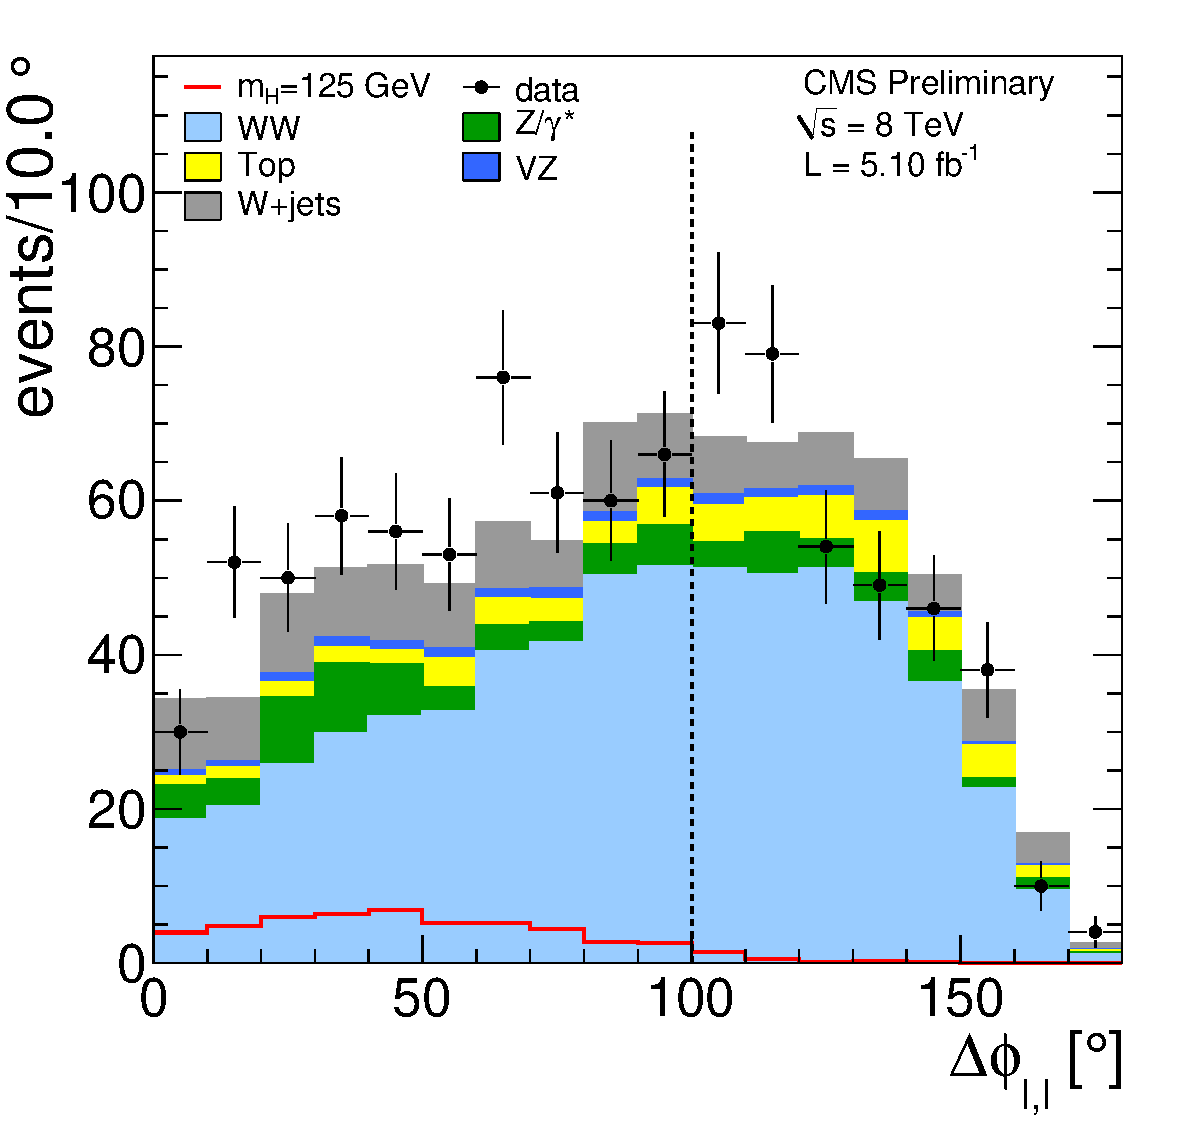
\includegraphics[width=0.49\textwidth]{dPhi_N-2_mh125_nj0.pdf}
   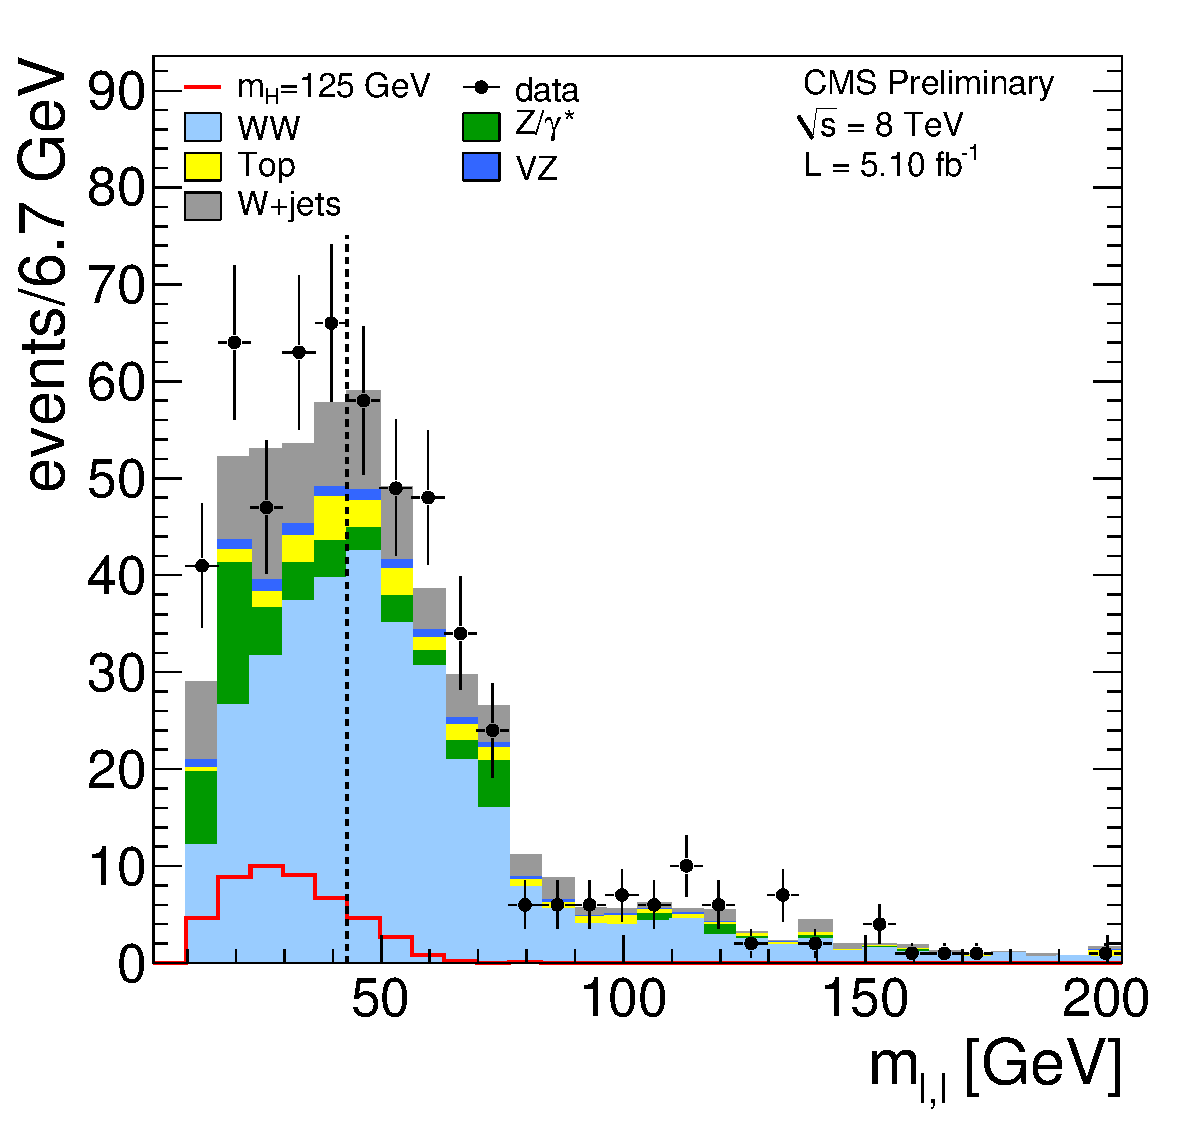
\includegraphics[width=0.49\textwidth]{dilepmass_N-1_mh125_nj0.pdf}
	\caption{Distributions of $\delphill$ (left) and dilepton mass
          (right) in the 0-jet category, for a $\mHi=125$ GeV SM Higgs
          boson and for the main backgrounds.  The cut-based $\hww$
          selection, except for the requirements on the $\delphill$
          and the dilepton mass, is applied (left) and dilepton mass (right). The vertical
          lines indicate the cut values.}  \label{fig:dphillHWW}
\end{center}
\end{figure}

The 2-jet category is mainly sensitive to the vector boson fusion
(VBF) production mode \cite{Ciccolini:2007jr}, whose cross section is
roughly ten times smaller than that of the gluon-gluon fusion mode.
The VBF signal can be extracted using extra selection criteria,
providing additional search sensitivity.  The $\hww$ events from VBF
production are characterized by a pair of energetic forward-backward
jets and very little hadronic activity in the rest of the event.
Events passing the $\WW$ criteria are further required to satisfy
$\pt>30$ GeV for both leading jets, with no jets above this threshold
present in the pseudorapidity region between the two leading jets. The
two leptons are required to be within the pseudorapidity region
defined by the two jets.  To reject the main background from top-quark
decays, two additional requirements are applied to the two jets, $j_1$
and $j_2$: $|\Delta\eta (j_1,j_2)| > 3.5$ and $m_{j_1j_2}
>450$ GeV. In addition, $m_\mathrm{T}$ is required to be larger than
30 GeV and smaller than the Higgs mass hypothesis. Finally, a
$\mHi$ dependent upper limit on the dilepton mass is applied.

A combination of techniques is used to determine the contributions
from the background processes that remain after the Higgs selection.
Where feasible, background contributions are estimated directly from
data, avoiding large uncertainties related to the simulation of these
sources. The remaining contributions taken from simulation are small.
The $\Wjets$ and QCD multi-jet backgrounds arise from leptonic decays
of heavy quarks, hadrons misidentified as leptons, and electrons from
photon conversion. The estimate of these contributions is derived
directly from data using a control sample of events in which one
lepton passes the standard criteria and the other does not, but
instead satisfies a relaxed set of requirements, resulting in a
``tight-fail'' sample. The efficiency, for a jet that satisfies the
loose selection to pass the tight selection is determined using data
from an independent multi-jet event sample dominated by non-prompt
leptons and used to extrapolate the ``tight-fail'' counts into the
signal region (``tight-tight'' sample).  Systematic uncertainties of
this method is estimated to be about 36\%.  The normalization of the
top-quark background is estimated from data as well by counting the
number of top-tagged events and applying the corresponding top-tagging
efficiency measured on data with one b-tagged jet.  The main
uncertainty comes from the statistical uncertainty in the control
sample and from the systematic uncertainties related to the
measurement of the tagging efficiency (about 20\% in the 0-jet
category and about 5\% in the 1-jet category).  For the low-mass
$\hww$ signal region, $\mHi \leq 200$ GeV, the non-resonant $\WW$
contribution is estimated from data. This contribution is measured
using events with a dilepton mass larger than 100~GeV, where the Higgs
boson signal contamination is negligible, and a simulation is used to
extrapolate into the signal region. The total uncertainty is about
10\%.  For larger Higgs boson masses there is a large overlap between
the non-resonant $\WW$ and Higgs boson signal, and simulation is used
for the estimation.  The $\dyll$ contribution to the $\Elp\Elm$ and
$\Mp\Mm$ final states is based on extrapolation from the observed
number of events with a dilepton mass within $\pm7.5$ GeV of the $\Z$
mass, where the residual background in that region is subtracted using
$\Elpm\Mmp$ events.  The largest uncertainty in the estimate is the
statistical uncertainty of the control sample, which is about 20\% to
50\%.  The $\dytt$ contamination is estimated using $\dyee$ and
$\Mp\Mm$ events selected in data, where the leptons are replaced with
simulated $\Tau$ decays, thus providing a better description of the
experimental conditions with respect to the simulation.  Finally, to
estimate the normalization of $\wgamma^{*}$ background contribution
from asymmetric virtual photon decays, where one lepton escapes
detection, a control sample of high purity $\wgamma^{*}$ events with
three reconstructed leptons is used. A measured factor of $1.6\pm0.5$
with respect to the leading order cross section is found.  Other minor
backgrounds from $\WZ$, $\ZZ$ (when the two selected leptons come from
different bosons) and $\wgamma$ are estimated from simulation.

%% The number of events observed and the expected number of events from
%% all processes after the $\WW$ selection, taking into account the data driven estimates,
%% are summarized in Table \ref{tab:wwselection_all}. 

%% \begin{table}[h!]
%%   \begin{center}                                                
%%   \caption{Observed number of events and background estimates for 
%%     an integrated luminosity of $\usedLumi$ after applying the $\WW$ selection requirements.
%%       Only statistical uncertainties on each estimate are reported.
%%    \label{tab:wwselection_all}}
%%   \begin{tabular}{c|c|c|c|c}
%% \hline
%%               & data             &  tot bkg.         & WW                & \ttbar+tW               \\ \hline
%%     0-jet bin & 1594             & 1501 $\pm$ 21    & 1046.1 $\pm$ 7.2   & 164.2 $\pm$ 5.4         \\
%%     1-jet bin & 1186             & 1162 $\pm$ 27    &  381.0 $\pm$ 4.0   & 527.3 $\pm$ 8.4         \\
%%     2-jet bin & 1295             & 1412 $\pm$ 24    &  177.0 $\pm$ 2.8   & 886.5 $\pm$ 11.1 \\ \hline  
%%               & W+jets           & WZ+ZZ            & Z$/\gamma^*$       & W+$\gamma^{(*)}$     \\ \hline
%%     0-jet bin & 158.2 $\pm$ 7.1  & 32.6 $\pm$ 0.6   & 73 $\pm$ 17        & 27.1 $\pm$ 3.9 \\
%%     1-jet bin & 122.6 $\pm$ 6.7  & 30.3 $\pm$ 0.6   & 77 $\pm$ 24        & 23.7 $\pm$ 5.2 \\
%%     2-jet bin &  94.9 $\pm$ 6.4  & 20.8 $\pm$ 0.5   & 227 $\pm$ 20       & 5.6 $\pm$ 2.1 \\ \hline
%%   \end{tabular}
%%   \end{center}
%% \end{table}

%%%%%%%%%%%%%%%%%%%%%%%%%%%%%%%%%%%%%%%%%%%%%%%%%%%%%%%%%%%%%%%%%%%%%%%%%%%%%%%
\section{$\Hi \to \WW \to \ell\nu qq$ search strategy}
\label{sec:hwwlnu2q}
%%%%%%%%%%%%%%%%%%%%%%%%%%%%%%%%%%%%%%%%%%%%%%%%%%%%%%%%%%%%%%%%%%%%%%%%%%%%%%%

The combination of the two highest $\pt$ jets is chosen as the
hadronic W candidate.  The events with the incorrect dijet combination
comprise a broad non-peaking background in the WW mass spectrum.  The
leptonic W candidate is reconstructed from the lepton plus $\MET$
system. We require $\MET>25$ (30) GeV for each event in the muon
(electron) data.  The transverse mass of the leptonic W candidate is
defined as {\small $\MT \equiv
  \sqrt{2~p_\mathrm{T}^l~\MET~(1-\cos(\phi_l-\phi_{\MET}))}$}, where
$\phi_l$ and $\phi_{\MET}$ are the azimuthal angles of the lepton and
$\MET$, respectively.  The transverse mass $\MT$ is required to be
larger than 30 GeV.  The main background after this selection is due
to the production of W bosons in association with jets.  The
requirement 65 GeV $< m_{jj} <$ 95 GeV, which keeps about 80\% of the
signal events, is subsequently applied in order to reduce this
background.  To exploit the differences in kinematics between signal
and background, a likelihood discriminant is constructed that
incorporates a set of five angular variables that best distinguishes
the Higgs signal from the W+jets background, optimized for several
Higgs mass points.  The four-body mass shape of the W+jets
contribution is extracted from data as a mixture of the shape measured
in two signal-free regions: 95 GeV $<m_{jj}<$ 115 GeV and 55 GeV
$<m_{jj}<$ 65 GeV.  The four-body mass shape for multi-jet background
events is obtained from data as well, by selecting a control sample of
non-isolated leptons and relaxing the $\MET$ threshold and
identification requirements.  For all the other backgrounds the Monte
Carlo prediction is used.  The $m_{\ell\nu{}jj}$ invariant mass
distribution in the signal region is shown in
Figure~\ref{fig:mlvjj_mH350} for muon plus 2-jet final state with
selections optimized for Higgs mass hypotheses of 200 GeV, 300 GeV,
and 500 GeV.
%
\begin{figure}[!t]
  \centering
  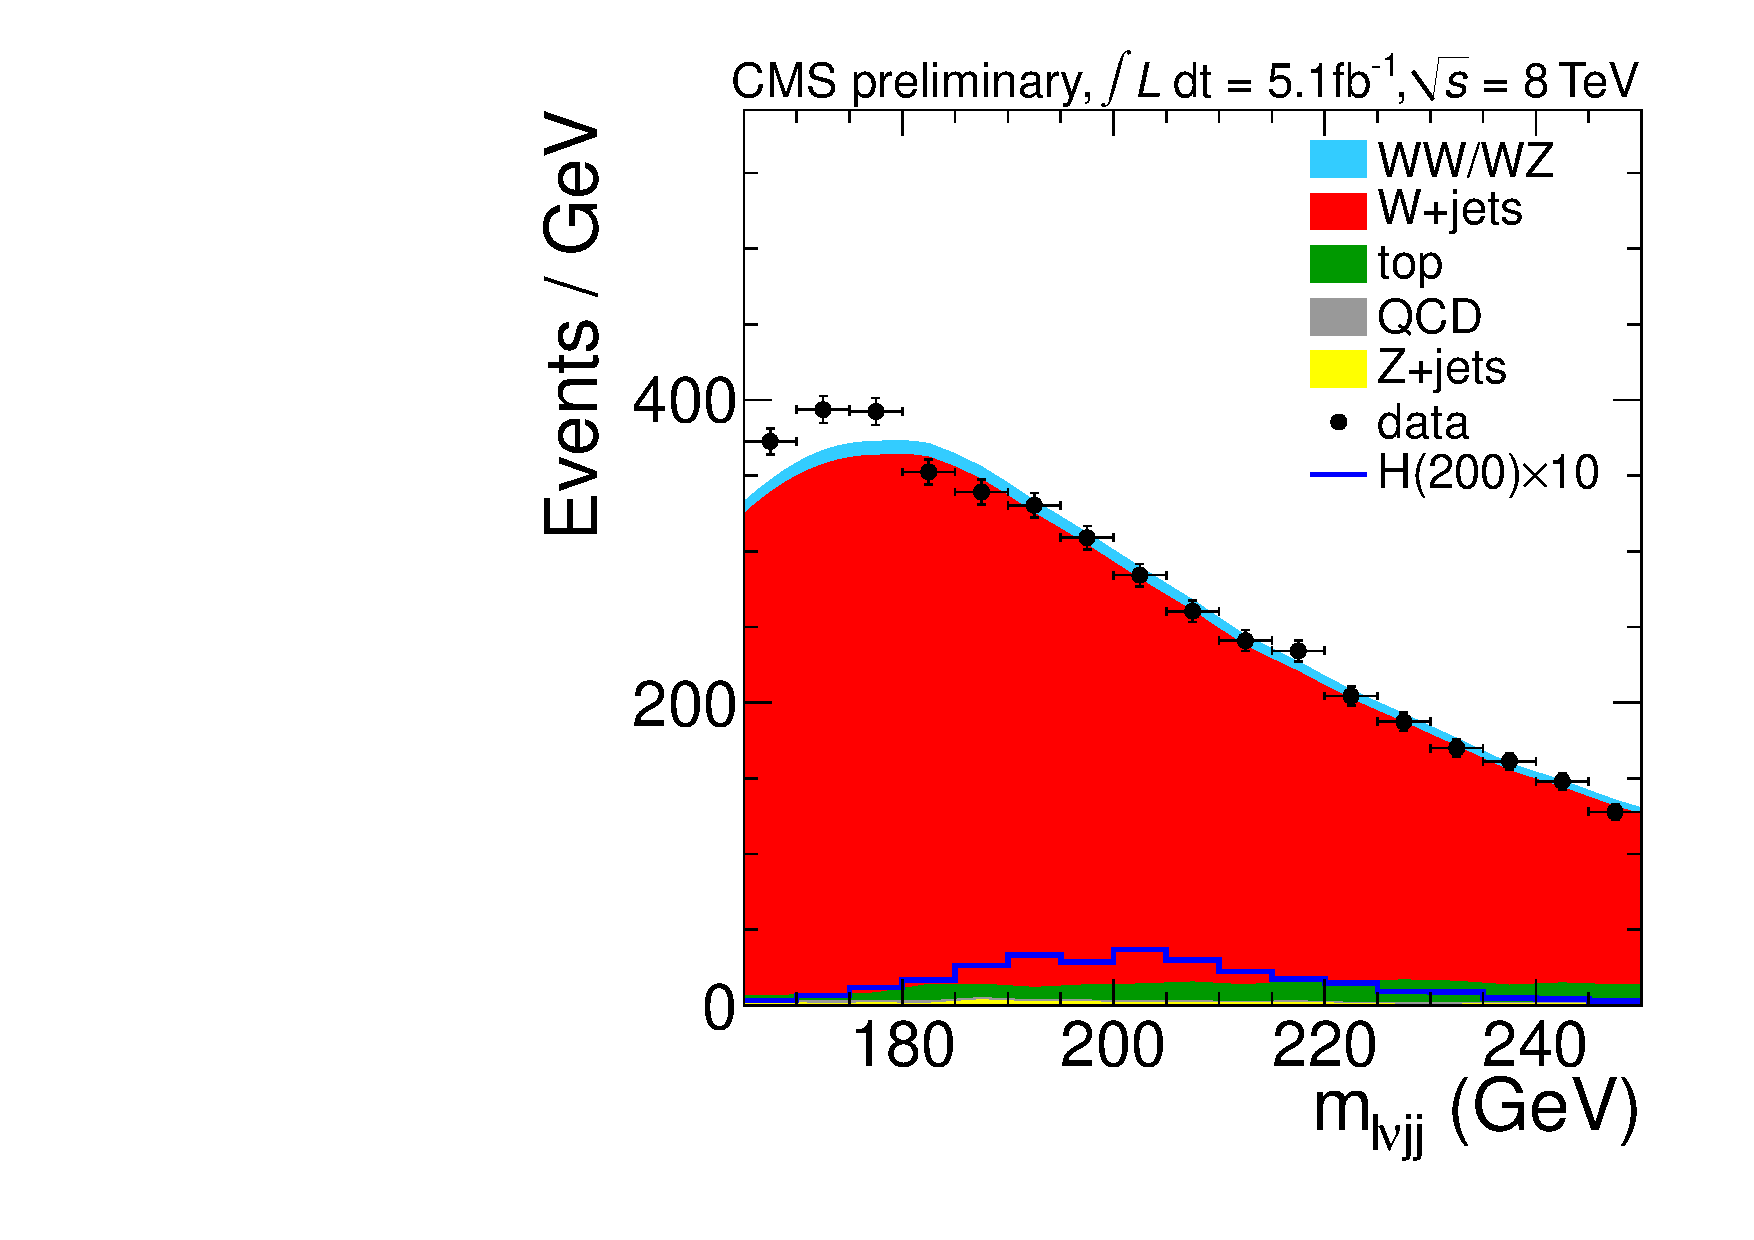
\includegraphics[width=0.32\textwidth]{H200_Mlvjj_Muon_2jets_Stacked.pdf}
  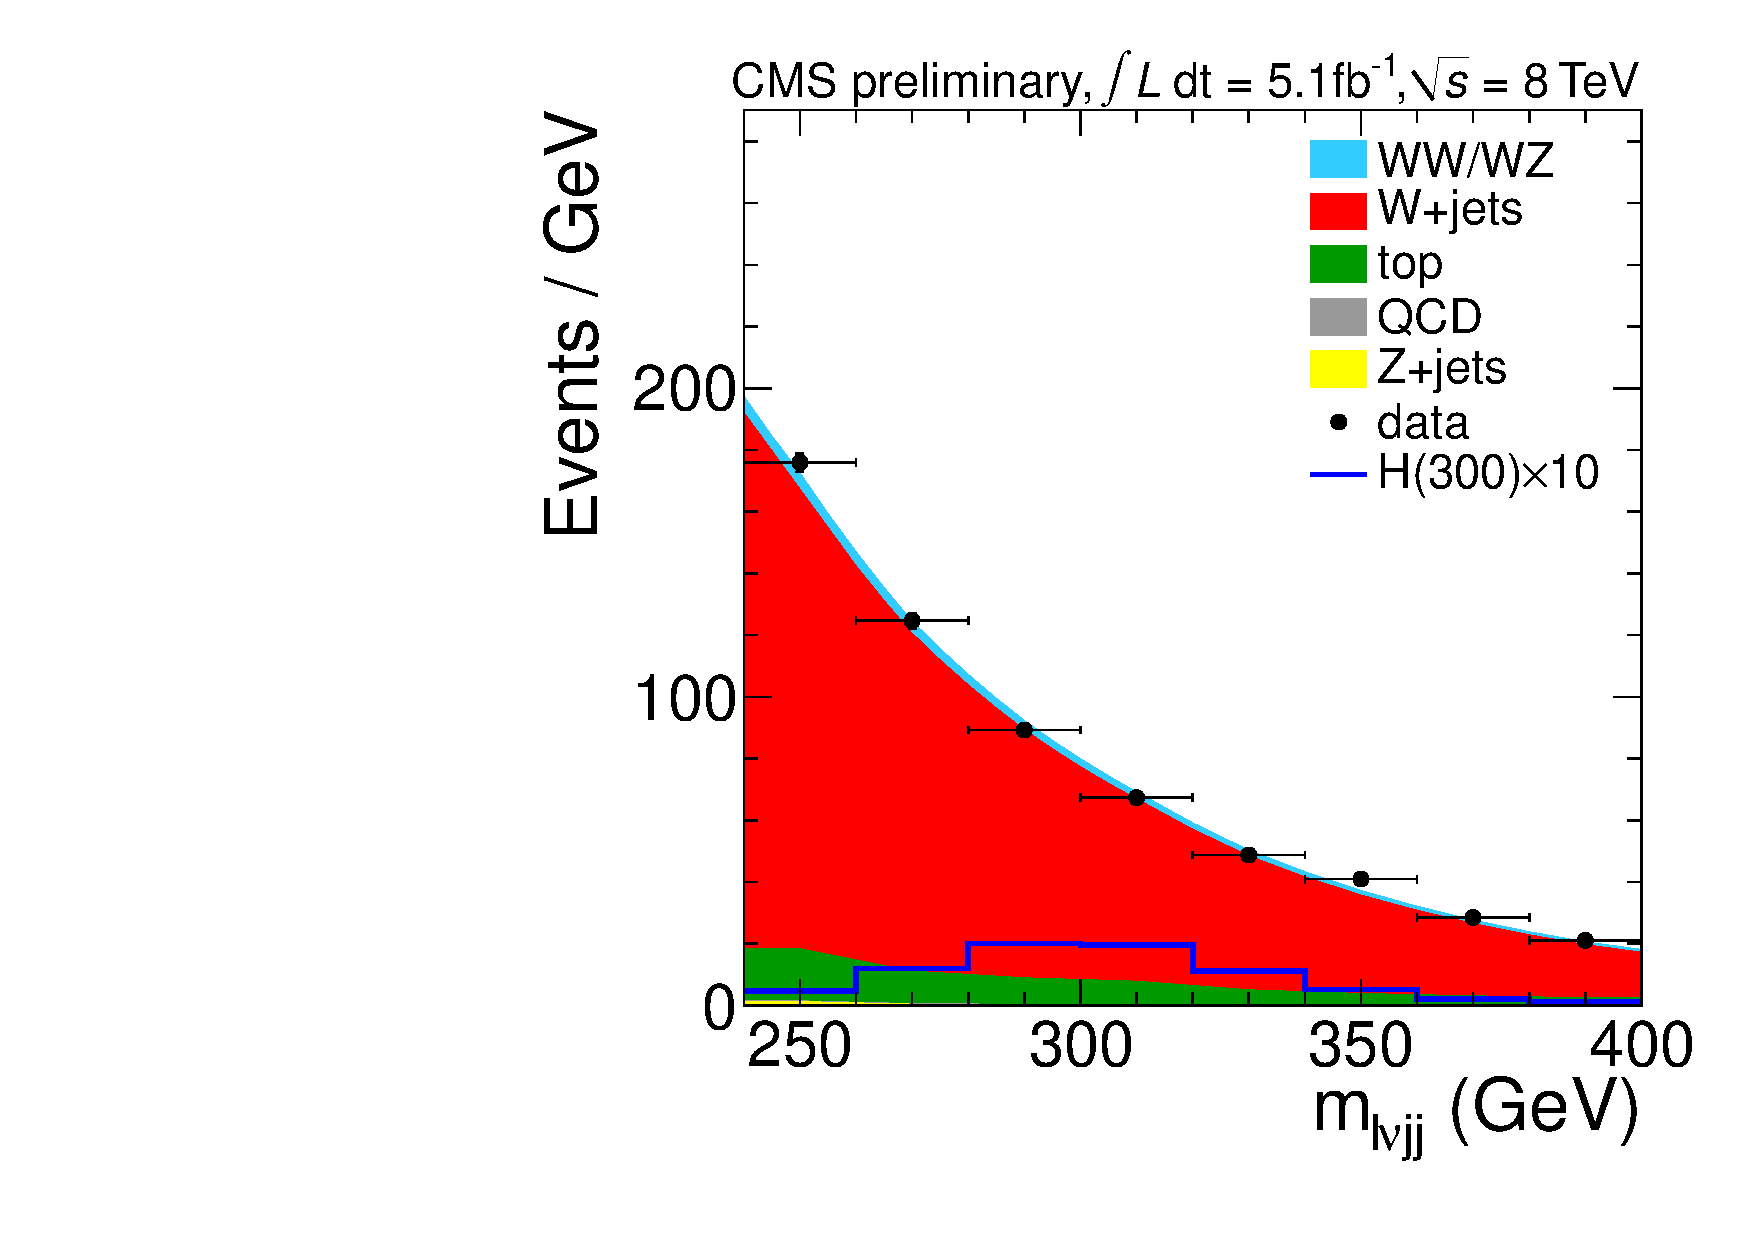
\includegraphics[width=0.32\textwidth]{H300_Mlvjj_Muon_2jets_Stacked.pdf}
  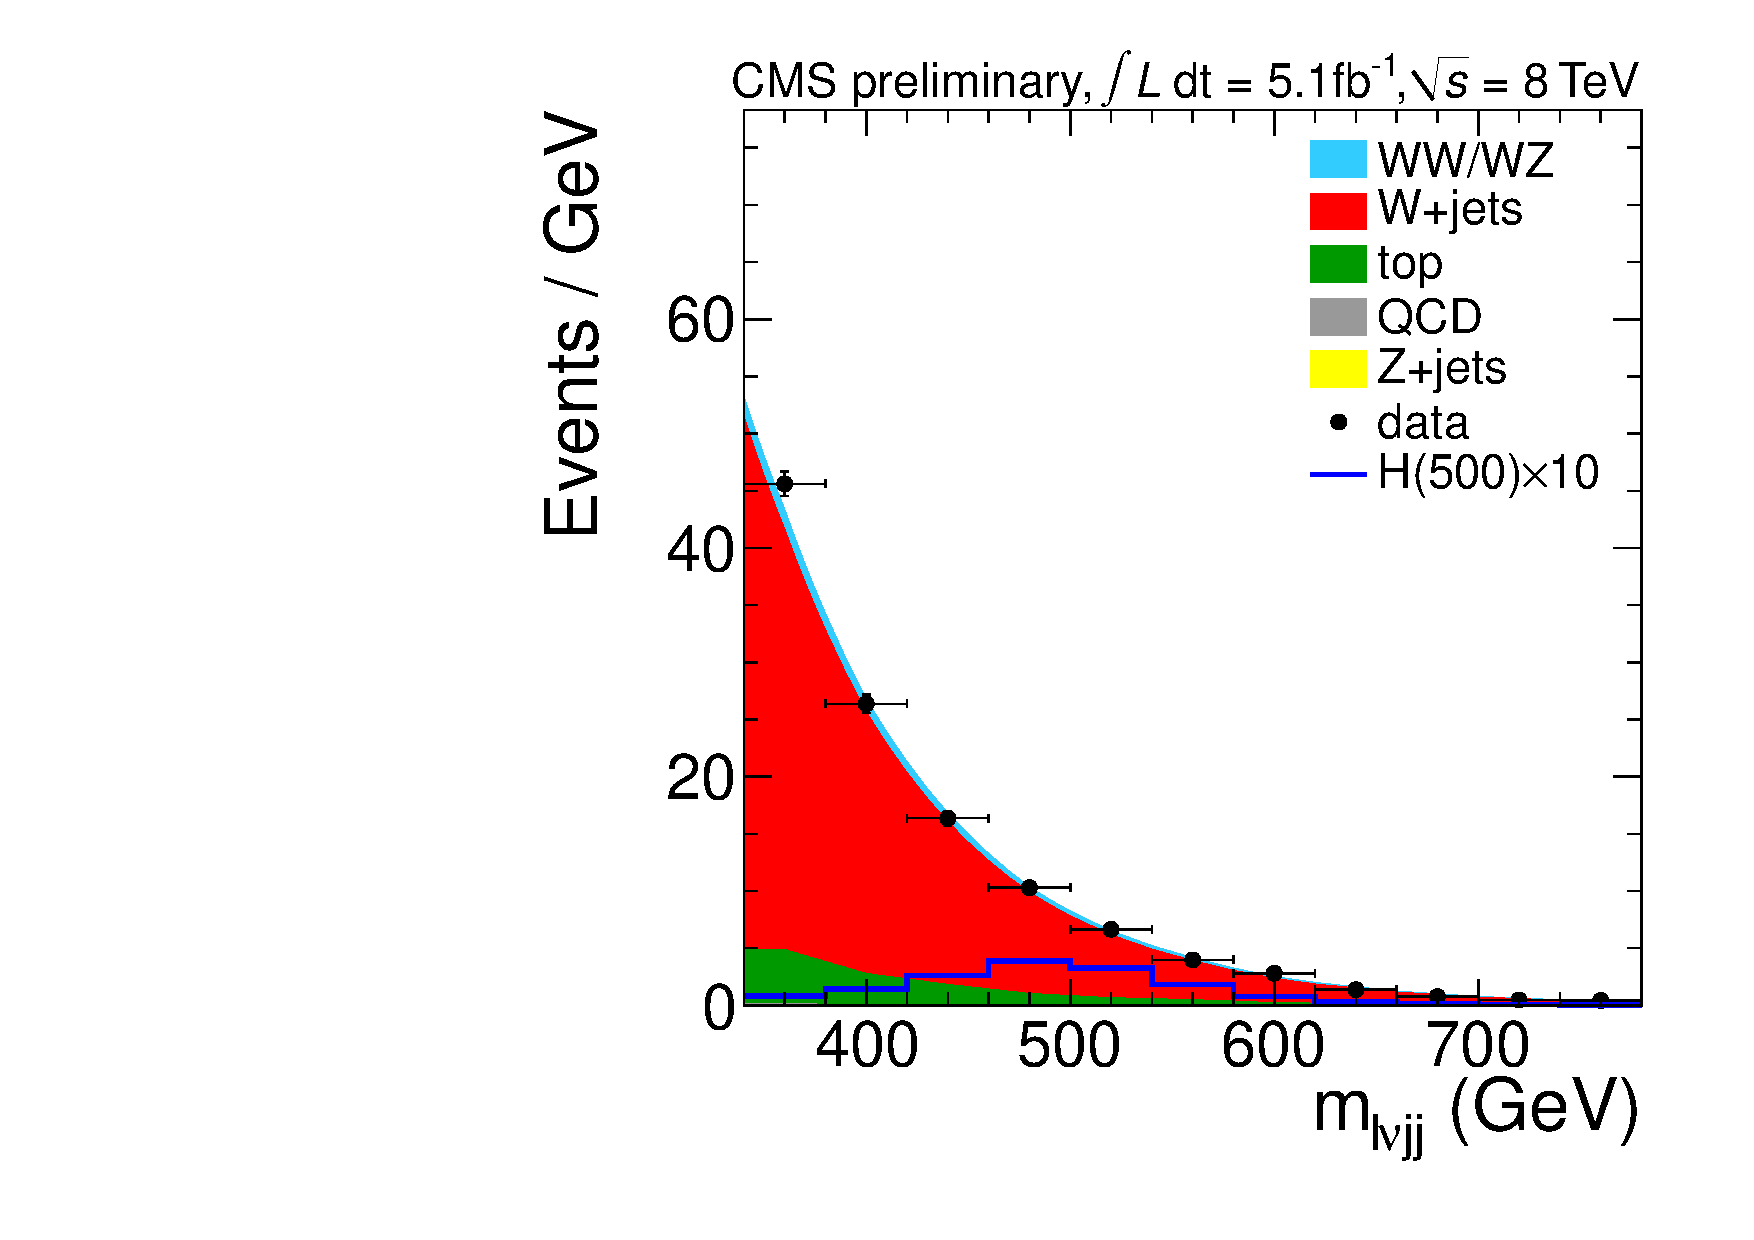
\includegraphics[width=0.32\textwidth]{H500_Mlvjj_Muon_2jets_Stacked.pdf}
  \caption{\label{fig:mlvjj_mH350} The WW invariant mass distribution
    with the fit projections in the signal region 65 GeV $<m_{jj}<$ 95
    GeV, for the muon 2-jet category, after selections optimized for
    the Higgs mass hypotheses of 200 GeV (left), 300 GeV (middle), and
    500 GeV (right).}
\end{figure}


%%%%%%%%%%%%%%%%%%%%%%%%%%%%%%%%%%%%%%%%%%%%%%%%%%%%%%%%%%%%%%%%%%%%%%%%%%%%%%%
\section{Results}
\label{sec:results}
%%%%%%%%%%%%%%%%%%%%%%%%%%%%%%%%%%%%%%%%%%%%%%%%%%%%%%%%%%%%%%%%%%%%%%%%%%%%%%%
Upper limits are derived on the ratio of the product of the Higgs
boson production cross section and the $\Hi \to \WW$ branching
fraction, $\sigma_{\Hi} \times \mathrm{BR}(\Hi \to \WW)$, and the SM
Higgs expectation, $\sigma/\sigma_\mathrm{SM}$.  To compute the upper
limits the modified frequentist construction CL$_{s}$~\cite{Read} is
used.  The 95\% CL observed and expected median upper limits are shown
in Fig.~\ref{fig:xsLim}. The bands represent the $1 \sigma$ and $2
\sigma$ probability intervals around the expected limit.  The 8~TeV
$\WW \to \ell\nu\ell\nu$ analysis excludes the presence of a Higgs
boson with mass in the range 135--198~GeV at 95\% CL, while the
expected exclusion limit in the hypothesis of background only is
128--250~GeV. With the addition of the 7~TeV analysis, a Higgs boson
with mass in the range 129--520~GeV is excluded at 95\% CL, while the
expected exclusion limit for the background only hypothesis is in the
range 122--450~GeV.  The observed (expected) upper limits are about
2.2 (1.2) times the SM expectation for $\mHi=125$ GeV.  A small excess
of events is observed for hypothetical low Higgs boson masses, which
makes the observed limits weaker than the expected ones.  The expected
significance for a SM Higgs of mass 125 GeV is 2.4 $\sigma$ and the
observed significance is 1.6 $\sigma$.  Due to the poor mass
resolution of this channel the excess extends over a large mass range.

With the $\WW \to \ell\nu qq$ analysis, the presence of a SM Higgs
boson in the mass range $260-460$ GeV is excluded at 95\% CL by
analyzing 8 TeV data.  Combining with 7 TeV results, a SM Higgs boson
is excluded in the mass range $230-480$ GeV, at 95\% confidence
level. The results are shown in Fig.~\ref{fig:xsLim}.
%-----------------------------------------------------
\begin{figure}[htbp]
  \begin{center}
    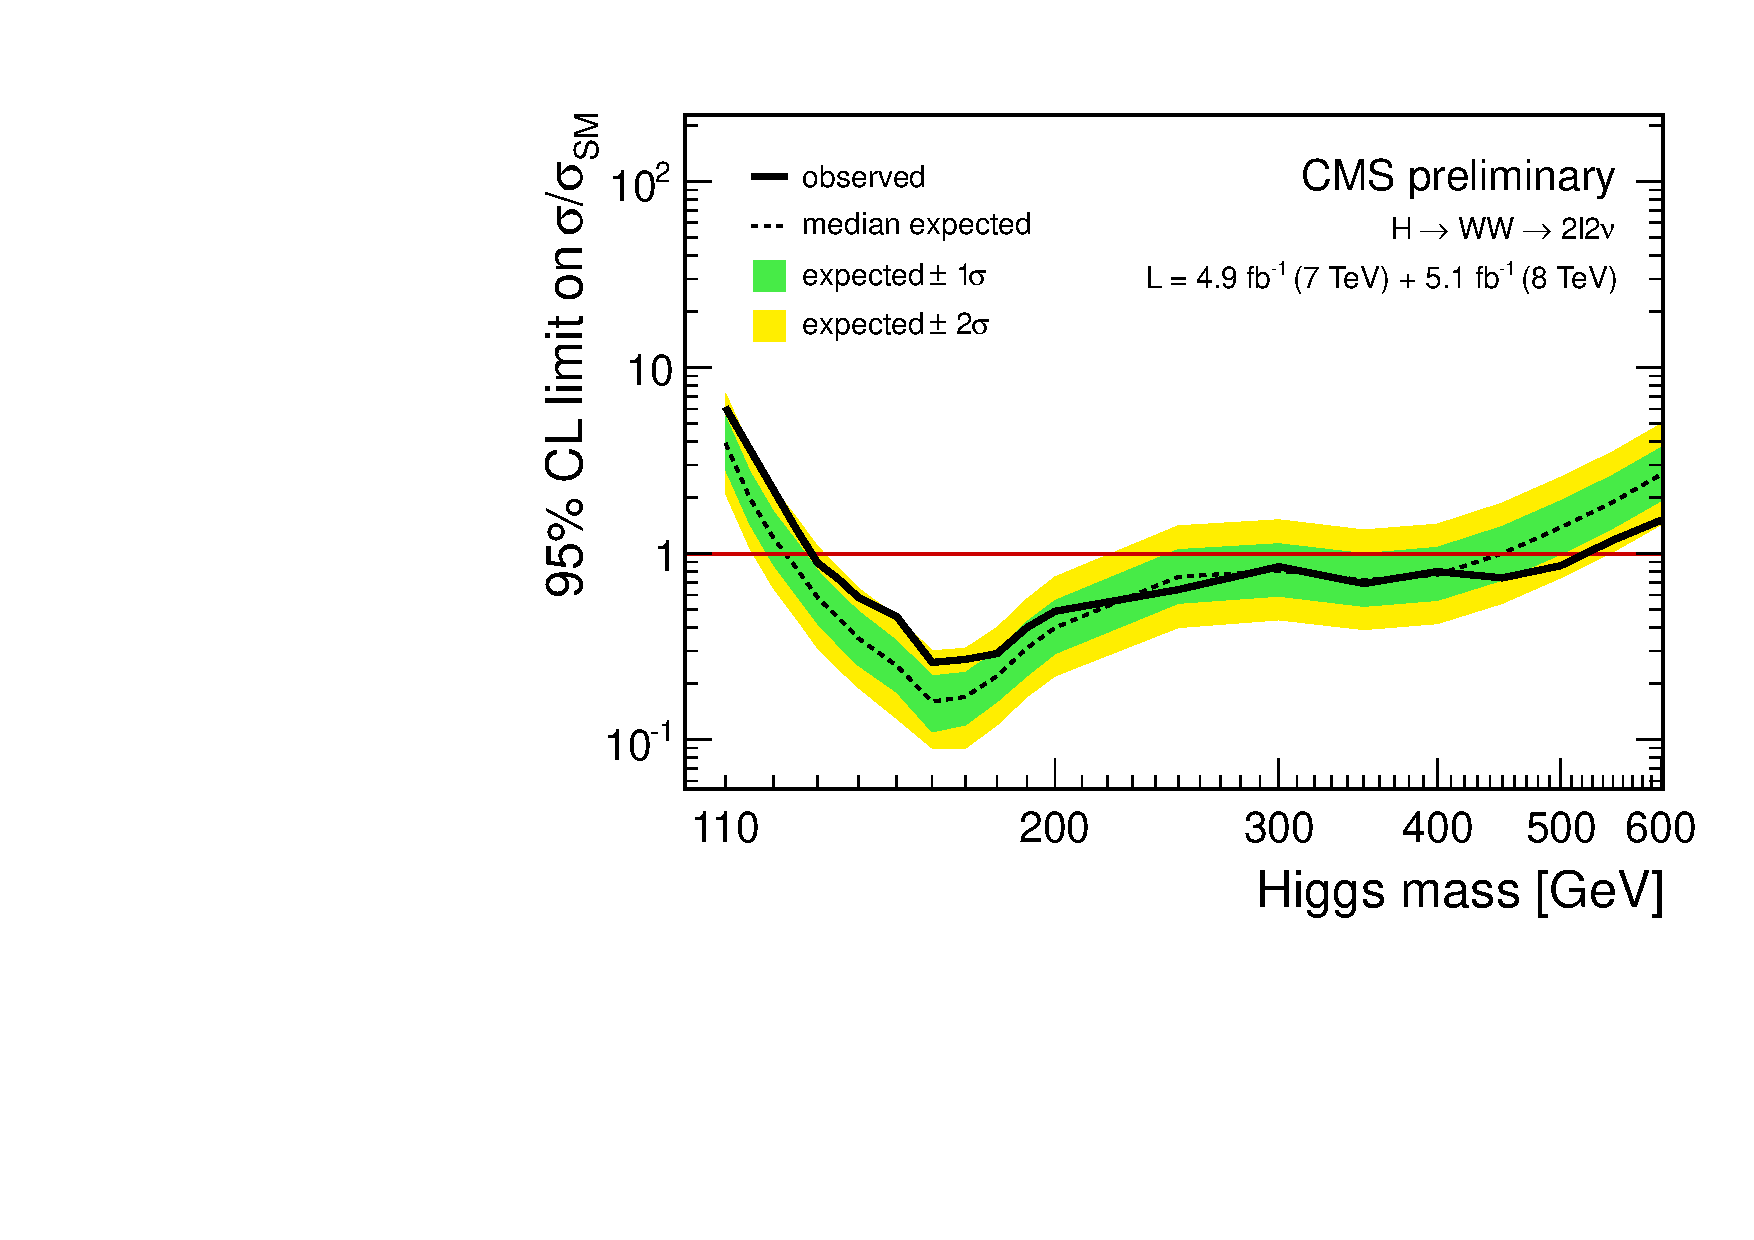
\includegraphics[width=0.49\textwidth]{limits_nj_shape7TeV_cut8TeV-CLs-asymptotic_logx_logy.pdf}
    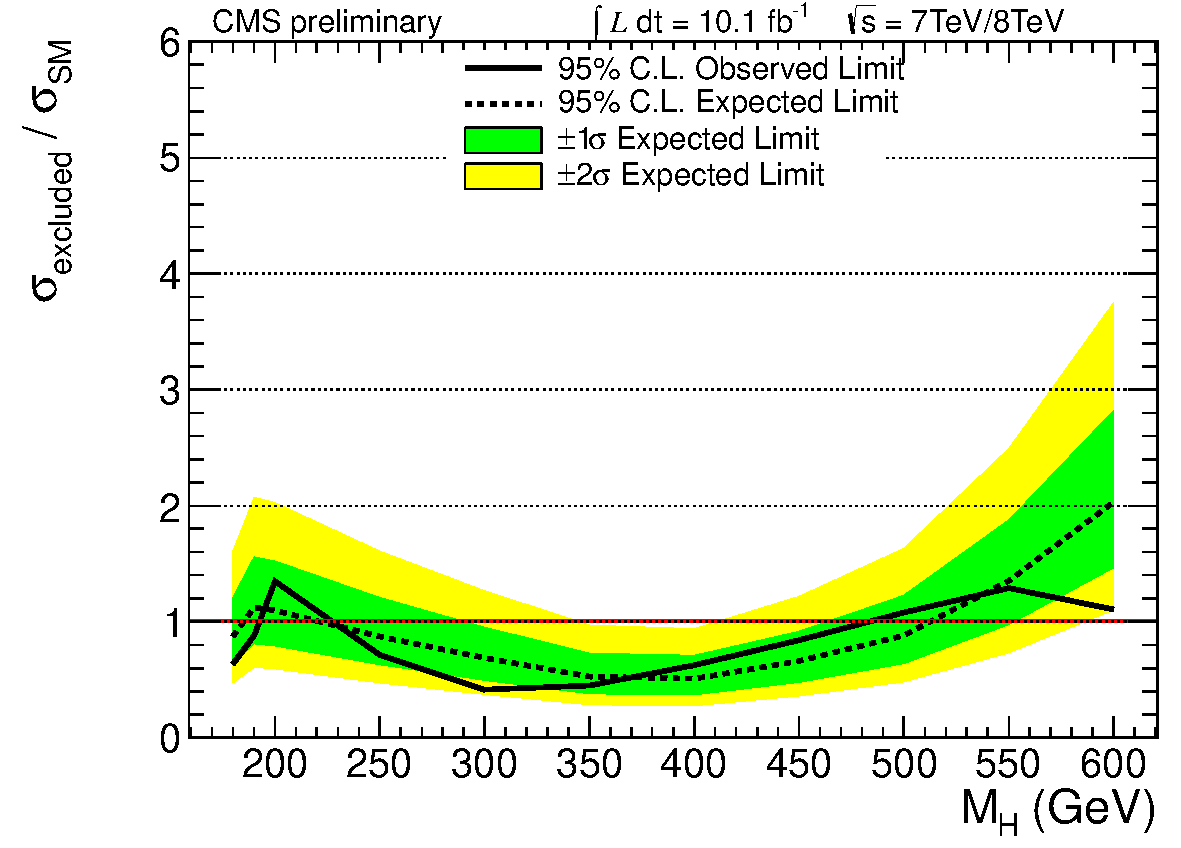
\includegraphics[width=0.49\textwidth]{limit_7and8tevcombined.pdf}
    \caption{Expected and observed 95\% CL upper limits on the cross
      section times branching fraction, $\sigma_{\Hi} \times
      \mathrm{BR}(\Hi \to \WW)$, relative to the SM Higgs expectation,
      using the combined 7 TeV and 8 TeV data for $WW \to
      \ell\nu\ell\nu$ analysis (left) and $\WW \to \ell\nu qq$
      analysis (right).  Results are obtained using the CL$_{s}$
      approach. \label{fig:xsLim}}
  \end{center}
\end{figure}
%-----------------------------------------------------



\begin{thebibliography}{99}
\bibitem{Higgs1} 
  P.~W.~Higgs,
  %``Broken Symmetries and the Masses of Gauge Bosons,''
  Phys.\ Rev.\ Lett.\  {\bf 13}, 508 (1964).
  %%CITATION = PRLTA,13,508;%%

%\cite{Englert:1964et}
\bibitem{Higgs2} 
  F.~Englert and R.~Brout,
  %``Broken Symmetry and the Mass of Gauge Vector Mesons,''
  Phys.\ Rev.\ Lett.\  {\bf 13}, 321 (1964).
  %%CITATION = PRLTA,13,321;%%

%\cite{Chatrchyan:2008aa}
\bibitem{CMSdetector} 
  S.~Chatrchyan {\it et al.}  [CMS Collaboration],
  %``The CMS experiment at the CERN LHC,''
  JINST {\bf 3}, S08004 (2008).
  %%CITATION = JINST,3,S08004;%%

%\cite{Chatrchyan:2012ty}
\bibitem{HWW2011} 
  S.~Chatrchyan {\it et al.}  [CMS Collaboration],
  %``Search for the standard model Higgs boson decaying to a W pair in the fully leptonic final state in pp collisions at sqrt(s) = 7 TeV,''
  Phys.\ Lett.\ B {\bf 710}, 91 (2012)
  %%CITATION = ARXIV:1202.1489;%%

\bibitem{egmpas} 
  [CMS Collaboration],
  %``Electron reconstruction and identification at sqrt(s) = 7 TeV,''
  CMS-PAS-EGM-10-004.
  %%CITATION = CMS-PAS-EGM-10-004;%%

\bibitem{antikt} 
  M.~Cacciari, G.~P.~Salam and G.~Soyez,
  %``The Anti-k(t) jet clustering algorithm,''
  JHEP {\bf 0804}, 063 (2008)
  %%CITATION = ARXIV:0802.1189;%%

%\cite{}
\bibitem{btag} 
  [CMS Collaboration],
  %``Algorithms for b Jet identification in CMS,''
  CMS-PAS-BTV-09-001.
  %%CITATION = CMS-PAS-BTV-09-001;%%

%\cite{Ciccolini:2007jr}
\bibitem{Ciccolini:2007jr} 
  M.~Ciccolini, A.~Denner and S.~Dittmaier,
  %``Strong and electroweak corrections to the production of Higgs + 2jets via weak interactions at the LHC,''
  Phys.\ Rev.\ Lett.\  {\bf 99}, 161803 (2007)
  %%CITATION = ARXIV:0707.0381;%%

%\cite{Read:2002hq}
\bibitem{Read} 
  A.~L.~Read,
  %``Presentation of search results: The CL(s) technique,''
  J.\ Phys.\ G {\bf 28}, 2693 (2002).


\end{thebibliography}

\end{document}


